% Diagrama vetorial do esquema de domínio do Ponto a Ponto (PaP), conferido no SQLite.
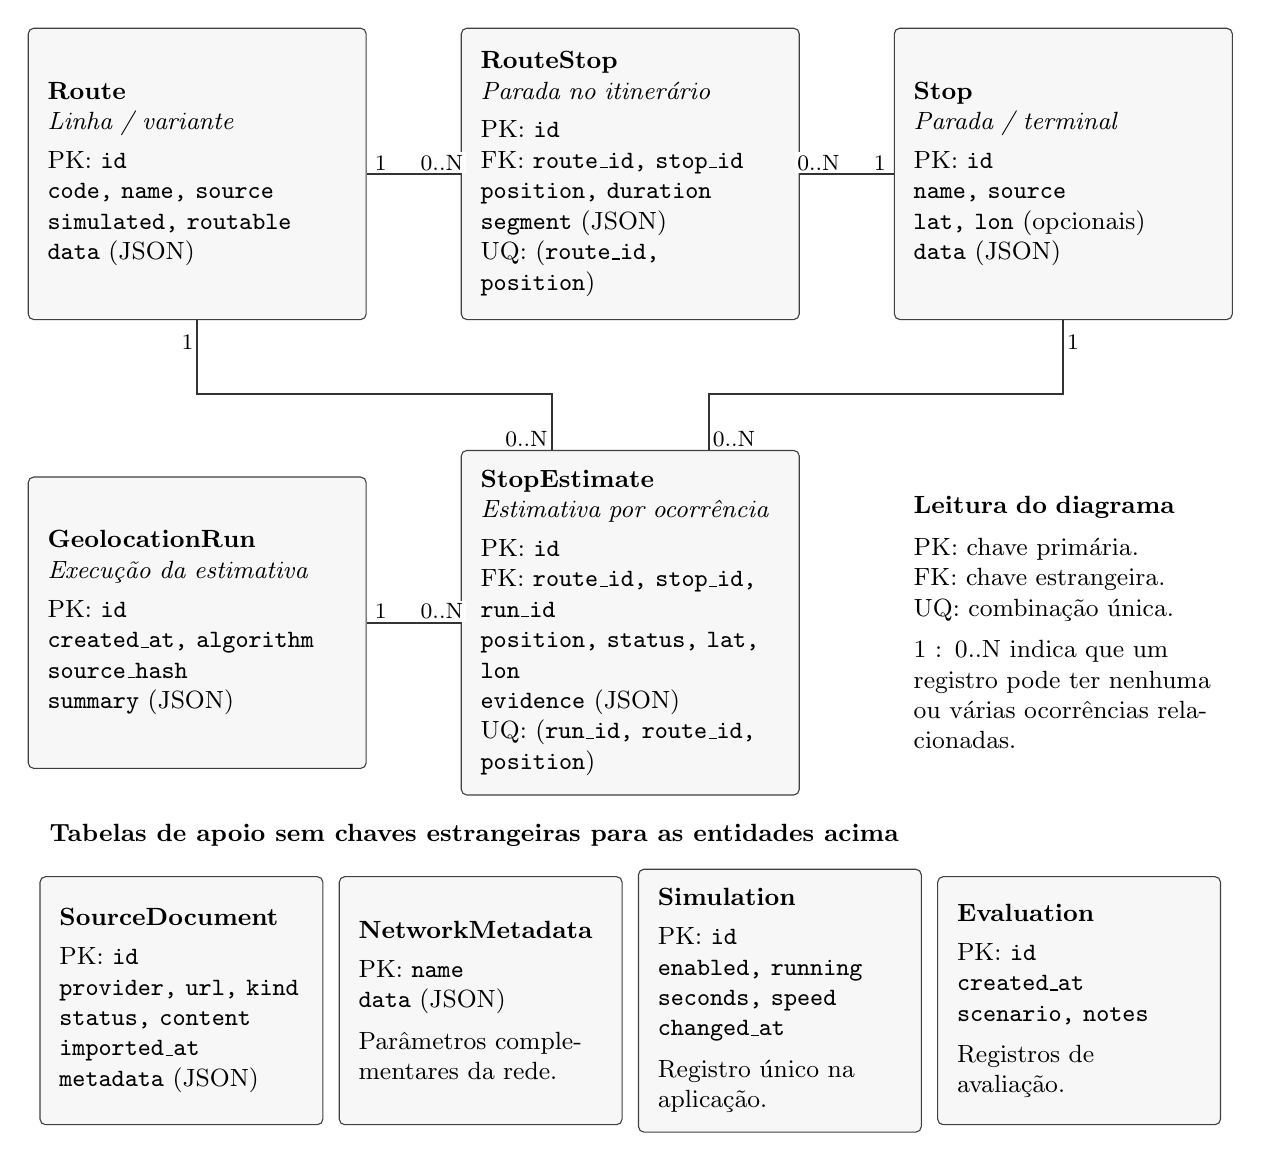
\begin{tikzpicture}[
  entity/.style={draw=black!75, fill=black!3, rounded corners=2pt,
    text width=3.8cm, inner sep=7pt, align=left, font=\fontsize{9}{11}\selectfont},
  support/.style={entity, text width=3.1cm, minimum height=3.15cm},
  relation/.style={draw=black!80, line width=0.7pt},
  cardinal/.style={font=\fontsize{8}{10}\selectfont, fill=white, inner sep=1pt}
]
\node[entity, minimum height=3.7cm] (route) at (0,0) {
  \textbf{Route}\\\textit{Linha / variante}\\[3pt]
  PK: \texttt{id}\\
  \texttt{code, name, source}\\
  \texttt{simulated, routable}\\
  \texttt{data} (JSON)
};
\node[entity, minimum height=3.7cm] (rs) at (5.5,0) {
  \textbf{RouteStop}\\\textit{Parada no itinerário}\\[3pt]
  PK: \texttt{id}\\
  FK: \texttt{route\_id, stop\_id}\\
  \texttt{position, duration}\\
  \texttt{segment} (JSON)\\
  UQ: (\texttt{route\_id, position})
};
\node[entity, minimum height=3.7cm] (stop) at (11,0) {
  \textbf{Stop}\\\textit{Parada / terminal}\\[3pt]
  PK: \texttt{id}\\
  \texttt{name, source}\\
  \texttt{lat, lon} (opcionais)\\
  \texttt{data} (JSON)
};
\node[entity, minimum height=3.7cm] (run) at (0,-5.7) {
  \textbf{GeolocationRun}\\\textit{Execução da estimativa}\\[3pt]
  PK: \texttt{id}\\
  \texttt{created\_at, algorithm}\\
  \texttt{source\_hash}\\
  \texttt{summary} (JSON)
};
\node[entity, minimum height=3.7cm] (estimate) at (5.5,-5.7) {
  \textbf{StopEstimate}\\\textit{Estimativa por ocorrência}\\[3pt]
  PK: \texttt{id}\\
  FK: \texttt{route\_id, stop\_id,}\\
  \texttt{run\_id}\\
  \texttt{position, status, lat, lon}\\
  \texttt{evidence} (JSON)\\
  UQ: (\texttt{run\_id, route\_id,}
  \texttt{position})
};
\draw[relation] (route.east) -- node[cardinal,above,pos=.15]{1}
  node[cardinal,above,pos=.8]{0..N} (rs.west);
\draw[relation] (stop.west) -- node[cardinal,above,pos=.15]{1}
  node[cardinal,above,pos=.8]{0..N} (rs.east);
\draw[relation] (run.east) -- node[cardinal,above,pos=.15]{1}
  node[cardinal,above,pos=.8]{0..N} (estimate.west);
\draw[relation] (route.south) -- node[cardinal,left,pos=.3]{1}
  (0,-2.8) -- (4.5,-2.8) -- node[cardinal,left,pos=.8]{0..N}
  ([xshift=-1cm]estimate.north);
\draw[relation] (stop.south) -- node[cardinal,right,pos=.3]{1}
  (11,-2.8) -- (6.5,-2.8) -- node[cardinal,right,pos=.8]{0..N}
  ([xshift=1cm]estimate.north);
\node[align=left,text width=3.8cm,font=\fontsize{9}{11}\selectfont] at (11,-5.7) {
  \textbf{Leitura do diagrama}\\[4pt]
  PK: chave primária.\\
  FK: chave estrangeira.\\
  UQ: combinação única.\\[4pt]
  1 : 0..N indica que um registro pode ter nenhuma ou várias ocorrências relacionadas.
};
\node[font=\fontsize{9}{11}\selectfont\bfseries,anchor=west] at (-2,-8.4) {Tabelas de apoio sem chaves estrangeiras para as entidades acima};
\node[support] at (-.2,-10.5) {
  \textbf{SourceDocument}\\[3pt]
  PK: \texttt{id}\\
  \texttt{provider, url, kind}\\
  \texttt{status, content}\\
  \texttt{imported\_at}\\
  \texttt{metadata} (JSON)
};
\node[support] at (3.6,-10.5) {
  \textbf{NetworkMetadata}\\[3pt]
  PK: \texttt{name}\\
  \texttt{data} (JSON)\\[4pt]
  Parâmetros complementares da rede.
};
\node[support] at (7.4,-10.5) {
  \textbf{Simulation}\\[3pt]
  PK: \texttt{id}\\
  \texttt{enabled, running}\\
  \texttt{seconds, speed}\\
  \texttt{changed\_at}\\[4pt]
  Registro único na aplicação.
};
\node[support] at (11.2,-10.5) {
  \textbf{Evaluation}\\[3pt]
  PK: \texttt{id}\\
  \texttt{created\_at}\\
  \texttt{scenario, notes}\\[4pt]
  Registros de avaliação.
};
\end{tikzpicture}
